\begin{frame}
\frametitle{Ce este CanSat?}
\begin{columns}[T]
    % \begin{column}{0.3\textwidth}
    %     \begin{tikzpicture}
    %         % \fill[lightblue] (0,0) rectangle (4,4);
    %         \node[white] at (2,2) {
    %         % \Huge \faSatellite};
    %         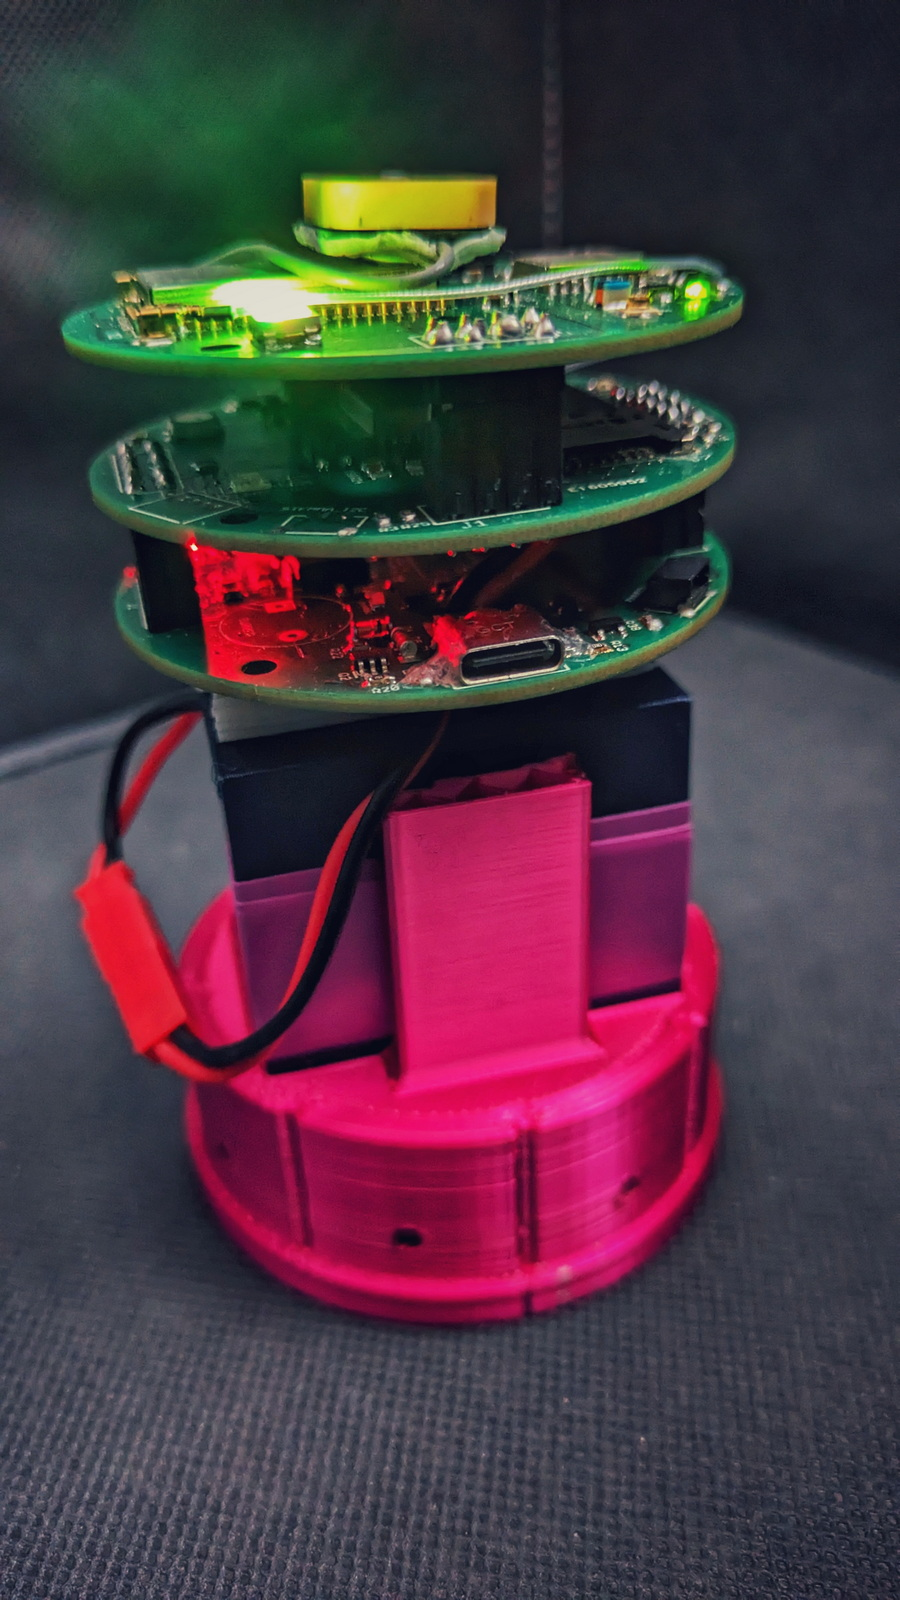
\includegraphics[height=5cm]{images/CDOSR-CanSat.jpeg}}
    %         % \node[white] at (2,1) {\small Un satelit într-o doză};
    %     \end{tikzpicture}
    % \end{column}
    \begin{column}{0.3\textwidth}
        \begin{center}  % Added center environment
            \vspace{-0.5cm}  % Add some vertical space from the top
            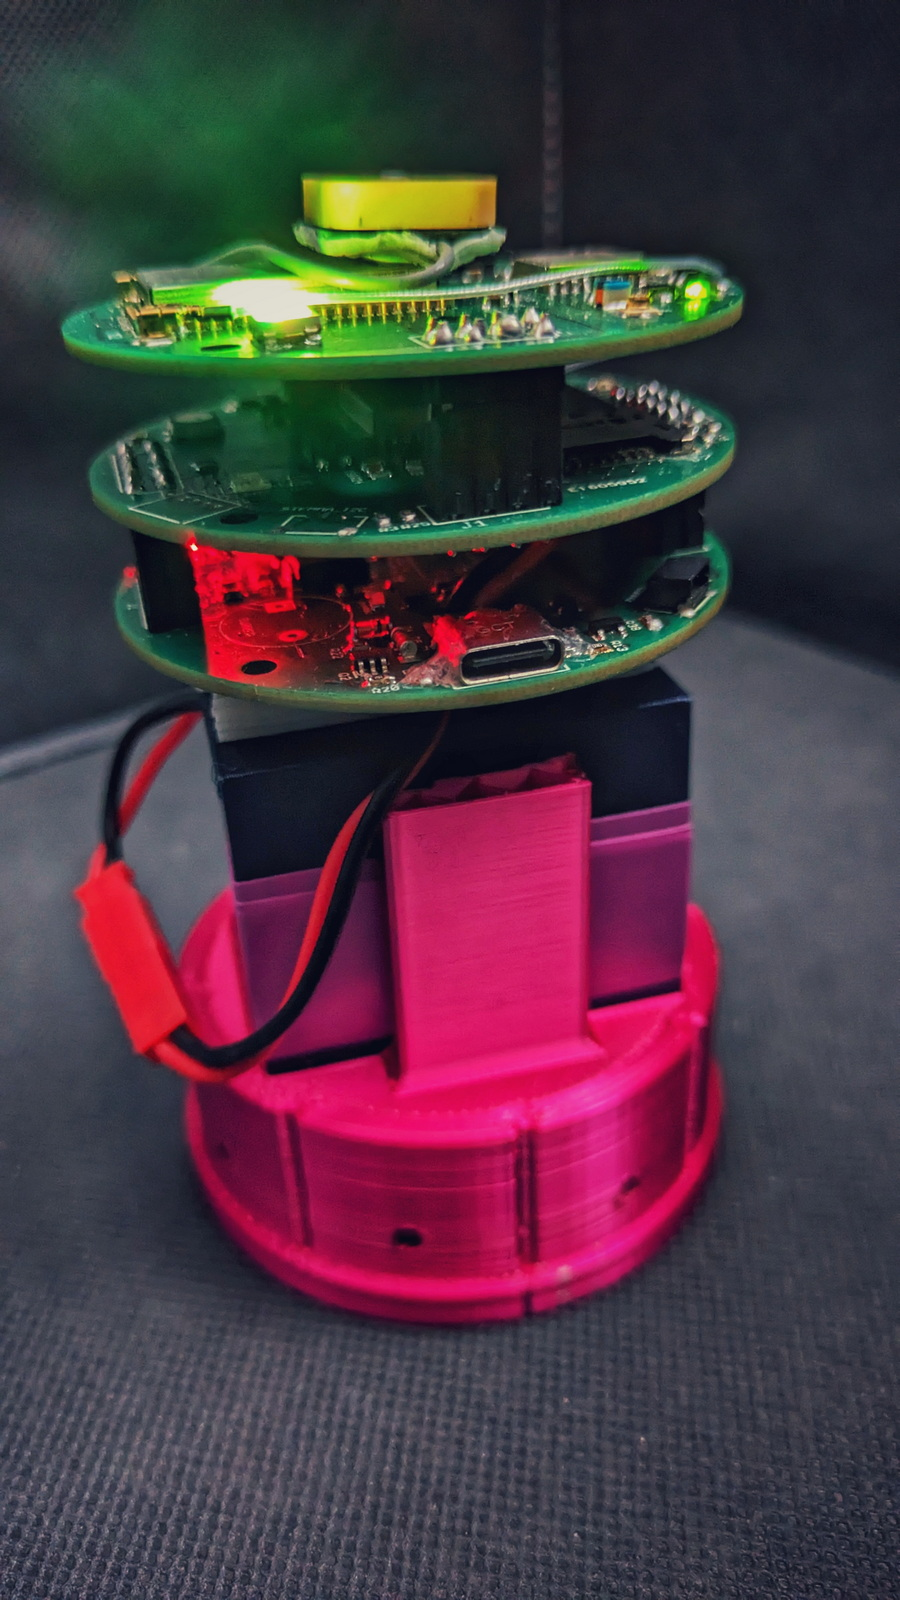
\includegraphics[height=5cm]{images/CDOSR-CanSat.jpeg}
        \end{center}
    \end{column}
    \begin{column}{0.7\textwidth}
     
        \textcolor{magenta}{\textbf{O misiune reală de satelit în formă miniaturizată}}\\[1em]
        {\usebeamerfont{column text}
        \begin{itemize}
            \item Se încadrează în volumul unei doze de suc de 330 ml
            \item Conține toate subsistemele unui satelit:
            {\usebeamerfont{column text}
                \begin{itemize}
                    \item Sisteme de alimentare (baterii, reglare)
                    \item Comunicații (radio telemetrie)
                    \item Senzori (temperatură, presiune, GPS)
                    \item Gestionarea și procesarea datelor
                    \item Sistem de recuperare (parașută)
                \end{itemize}
                }
            \item Simulează ciclul complet de viață al unei misiuni spațiale
        \end{itemize}
        }
    \end{column}
\end{columns}

\bcolorbar  % Adding the bottom color bar
\end{frame}